\section{Project Plan}
\label{sec:project_plan}

The project based UvA thesis milestones and executed using, Scrum sprints to build the thesis. This approach is suitable for computer-vision research because progress depends on iterative experimentation (dataset sourcing, pre processing, baseline definition, model selection, and evaluation), where results may require revising earlier decisions. Sprint planning supports incremental deliverables and frequent review while ensuring alignment with fixed submission deadlines.

\subsection{Timeline Overview}
Figure~\ref{fig:timeline_split} provides a high level overview. The timeline may be adjusted based on knowledge, data availability, and experimental outcomes.

\begin{figure}[t]
\centering
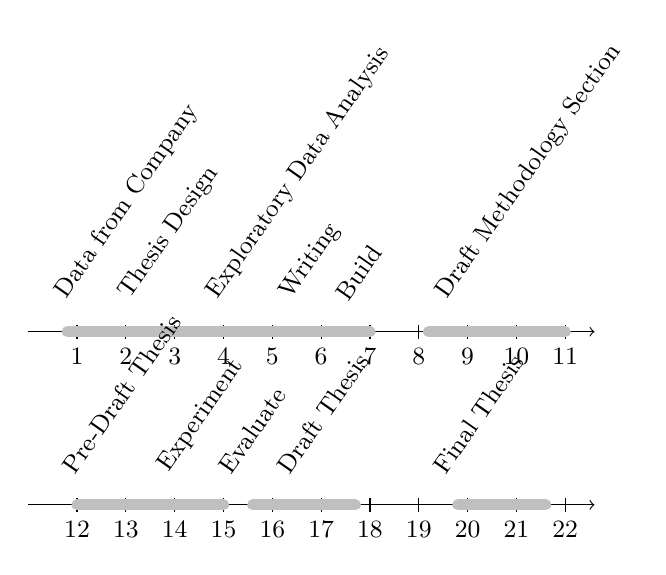
\begin{tikzpicture}[x=0.62cm,y=1cm, font=\small]

% ===== Top timeline: 1..11 =====
\draw[->] (0,0) -- (11.6,0);
\foreach \x in {1,...,11} {
  \draw (\x,0.09) -- (\x,-0.09);
  \node[below] at (\x,-0.09) {\x};
}
\node[rotate=55, anchor=south west] at (0.9,0.20) {Data from Company};
\node[rotate=55, anchor=south west] at (2.2,0.20) {Thesis Design};
\node[rotate=55, anchor=south west] at (4.0,0.20) {Exploratory Data Analysis};
\node[rotate=55, anchor=south west] at (5.5,0.20) {Writing};
\node[rotate=55, anchor=south west] at (6.6,0.20) {Build};
\node[rotate=55, anchor=south west] at (8.7,0.20) {Draft Methodology Section};

\draw[line width=4pt, gray!50, line cap=round] (0.8,0) -- (7.0,0);
\draw[line width=4pt, gray!50, line cap=round] (8.2,0) -- (11.0,0);

% ===== Bottom timeline: 12..22 =====
\begin{scope}[yshift=-2.2cm]
\draw[->] (0,0) -- (11.6,0);
\foreach \i [evaluate=\i as \lab using int(\i+11)] in {1,...,11} {
  \draw (\i,0.09) -- (\i,-0.09);
  \node[below] at (\i,-0.09) {\lab};
}
\node[rotate=55, anchor=south west] at (1.0,0.20) {Pre-Draft Thesis};
\node[rotate=55, anchor=south west] at (3.0,0.20) {Experiment};
\node[rotate=55, anchor=south west] at (4.2,0.20) {Evaluate};
\node[rotate=55, anchor=south west] at (5.4,0.20) {Draft Thesis};
\node[rotate=55, anchor=south west] at (8.6,0.20) {Final Thesis};

\draw[line width=4pt, gray!50, line cap=round] (1.0,0) -- (4.0,0);
\draw[line width=4pt, gray!50, line cap=round] (4.6,0) -- (6.7,0);
\draw[line width=4pt, gray!50, line cap=round] (8.8,0) -- (10.6,0);
\end{scope}

\end{tikzpicture}
\caption{Project timeline overview (split across two lines to fit the page).}
\label{fig:timeline_split}
\end{figure}

\subsection{Phases (Work Breakdown)}
The project is divided into four phases aligned with the thesis milestones:

\textbf{Phase 1: Thesis Design (January--February)} \\
\begin{itemize}
    \item Define research question, scope, and objectives.
    \item Conduct a literature review on change detection and computer vision.
    \item Collect datasets or identify image sources.
\end{itemize}

\textbf{Phase 2: Literature / exploratory work (March)} \\
\begin{itemize}
    \item Extend the literature review based on new methods.
    \item Refine research sub-questions.
    \item Explore dataset preparation and preprocessing requirements.
\end{itemize}

\textbf{Phase 3: Methodology Draft (April)} \\
\begin{itemize}
    \item Select a baseline computer vision technique.
    \item Define feature extraction, comparison strategy, and evaluation metrics.
    \item Draft setup and validation design.
\end{itemize}

\textbf{Phase 4: Prototype and Draft Thesis (May--June)} \\
\begin{itemize}
    \item Develop a working prototype.
    \item Evaluate results.
    \item Write thesis sections based on progress.
\end{itemize}

\subsection{Official Milestones (UvA Deadlines)}
\begin{itemize}
    \item \textbf{Before 10 Jan:} Register project on Datanose.
    \item \textbf{23 Feb (Canvas):} Thesis Design submission (4 pages).
    \item \textbf{Before 9 Mar (Datanose):} Supervisor-approved Thesis Design.
    \item \textbf{23 Mar (Canvas):} Exploratory Data Analysis / Literature Review milestone.
    \item \textbf{20 Apr (Canvas):} Draft Methodology Section.
    \item \textbf{19 May:} Midterm Evaluation.
    \item \textbf{25 May (Canvas):} Pre-Draft Thesis (preferably including initial Results).
    \item \textbf{15 Jun (Canvas):} Draft Thesis.
    \item \textbf{26 Jun (Datanose):} Final Thesis.
\end{itemize}

\subsection{Roadmap (Sprint-Level Plan)}
The planning is presented as a two-column list. Each sprint ends with a concrete deliverable and a review checkpoint.

\begin{center}
\small
\begin{tabular}{p{0.48\linewidth} p{0.48\linewidth}}
\textbf{Sprint 1 (Jan 5--18):} Thesis Design start; RQ/scope; register Datanose. &
\textbf{Sprint 2 (Jan 19--Feb 1):} Thesis Design iteration; refine gap + method motivation. \\
\textbf{Sprint 3 (Feb 2--15):} Finalise Thesis Design draft; submission preparation. &
\textbf{Sprint 4 (Feb 16--Mar 1):} Submit Thesis Design (23 Feb); begin data sourcing + EDA. \\
\textbf{Sprint 5 (Mar 2--15):} Literature extension; data collection + preprocessing. &
\textbf{Sprint 6 (Mar 16--29):} Submit March milestone (23 Mar); finalise dataset plan. \\
\textbf{Sprint 7 (Mar 30--Apr 12):} Draft Methodology; baselines + metrics + protocol. &
\textbf{Sprint 8 (Apr 13--Apr 26):} Submit Methodology (20 Apr); model selection buffer. \\
\textbf{Sprint 9 (Apr 27--May 10):} Build first model prototype. &
\textbf{Sprint 10 (May 11--May 24):} Experiments + refinement; Midterm (19 May); Pre-Draft (25 May). \\
\textbf{Sprint 11 (May 25--Jun 7):} Integrate results; write main thesis chapters. &
\textbf{Sprint 12 (Jun 8--Jun 21):} Draft Thesis (15 Jun); final revisions + formatting. \\
\multicolumn{2}{p{\linewidth}}{\textbf{Sprint 13 (Jun 22--Jun 30):} Final Thesis submission (26 Jun) + buffer.} \\
\end{tabular}
\end{center}
